\documentclass[11pt, oneside]{article} 
\usepackage{geometry}
\geometry{letterpaper} 
\usepackage{graphicx}
	
\usepackage{amssymb}
\usepackage{amsmath}
\usepackage{parskip}
\usepackage{color}
\usepackage{hyperref}

\graphicspath{{/Users/telliott_admin/Tex/png/}}
% \begin{center} 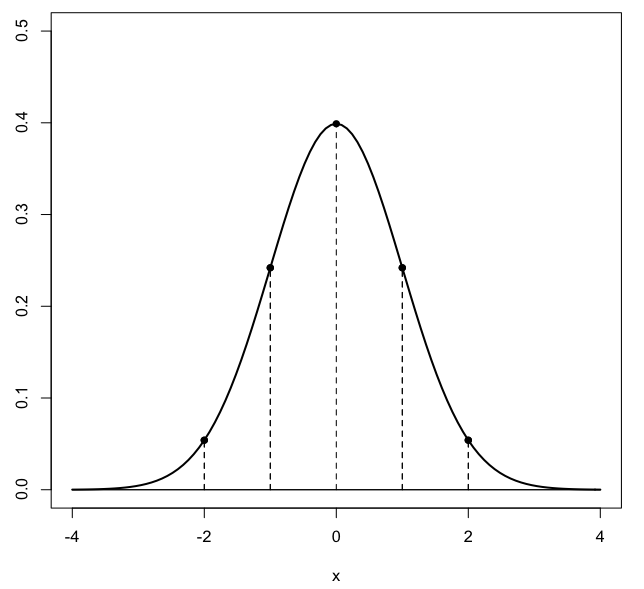
\includegraphics [scale=0.4] {gauss3.png} \end{center}

\title{Area of a circle}
\date{}

\begin{document}
\maketitle
\Large

This is a topic in geometry that comes even before the volume of the sphere, but I held off so as to start with Archimedes' most famous contribution.

We want the area of a circle.  Imagine dividing a circle into wedges, like you might do with a pizza.  Here, the pie has been divided into 16 parts.
\begin{center}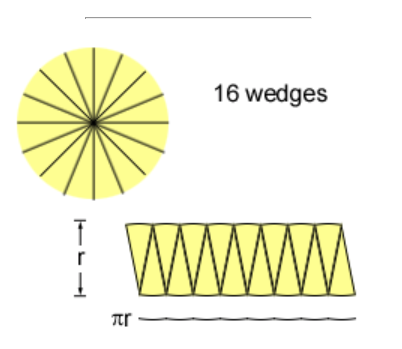
\includegraphics [scale=0.5] {circle_wedges.png}\end{center}

Since the pieces are triangular, it is easy to stack them next to each other with the bases and tips alternating, as shown.  Of course the bases are not straight, but have the same curvature as the edge of the circle.  

The length of the short side is the radius, $R$, and the length of the long side is approximately one-half the circumference so
\[ A = R \cdot \frac{1}{2} \cdot 2 \pi R = \pi R^2 \]

The trick is to imagine that we subdivide the circle into many slices.  If there are infinitely many  slices, the edges will be  straight and this calculation becomes exact.

According to wikipedia

\url{https://en.wikipedia.org/wiki/Area_of_a_circle}

Eudoxus of Cnidus, born in the 5th century (408 BCE), proved that the area of a circle, like that of regular polygons, is proportional to both horizontal and vertical dimensions, and thus is proportional to the radius squared.

Somewhat later, it became clear that for a regular polyhedron, the area is equal to one-half the perimeter times the altitude from the center to each side (called the apothem).  Allowing the polyhedron to achieve many, many sides, that formula gives $1/2 \cdot 2 \pi r \cdot r = \pi r^2$.

The proof we gave above is very much like one attributed to Leonardo da Vinci, among others.

Another idea is to remove concentric strips from the edge and stack them.
\begin{center}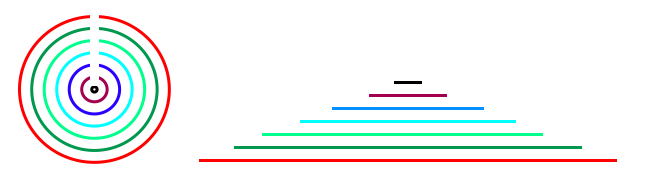
\includegraphics [scale=0.5] {circle_strips.png}\end{center}
We obtain a triangle of height $r$ and base $2 \pi r$ so its area is
\[ A = \frac{1}{2} \ 2 \pi r \cdot r = \pi r^2 \]

This proof was given by Archimedes and is found in his \emph{Measurement of a Circle}, proposition 1.  However, many sources, including

\url{http://www.math.tamu.edu/~dallen/masters/Greek/eudoxus.pdf}

attribute the proof to Eudoxus, who was perhaps the second most famous mathematician of antiquity, and a colleague of Plato in Athens.

(The proof can be skipped if you get bogged down): 

Let $A$ be the area of the circle and $T$ be the area of the triangle formed with base $2 \pi r$ and height $r$.  We will show that the following leads to a contradiction.  

Assume $A > T$.  That is, the difference $A - T$ is non-zero and positive:  $A - T > 0$.  

Using the methods described \hyperref[sec:Archimedes_and_pi]{\textbf{here}}, we know that it is possible to construct an inscribed polygon whose area differs from $A$ by \emph{as little as we please}.  Call that area $P$.  What we mean by \emph{as little as we please} is that $P$ can be made closer to $A$ than $T$ is.

Since this is an \emph{inscribed} polygon, we have
\[ A - P < A - T \]
\[ A + T < A + P \]
By this argument, we must have that $T < P$.  

But for an inscribed polygon the perimeter is certainly less than the circumference of the circle and its apothem (the vertical to the sides of the polygon) is less than the radius of the circle
\begin{center}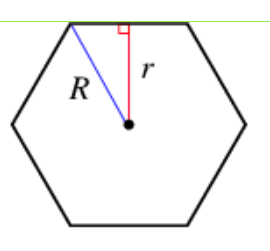
\includegraphics [scale=0.5] {apothem.png}\end{center}
In the figure, it must be that $r < R$.

By this argument, we must have that $P < T$.  However, we just got through showing that $T < P$.  We have reached a contradiction.  

Thus $A \ngtr T$.

A similar argument assuming $A < T$ also leads to a contradiction.  

Since $A$ is neither greater than nor smaller than $T$ it must be equal to $T$.
\[ A = T = \frac{1}{2} \cdot 2 \pi R \cdot R  = \pi R^2 \]

The analysis is taken from Dunham's \emph{Journey Through Genius}.  Here is a quote he presents from Plutarch, talking about Archimedes:

\begin{quote}It is not possible to find in all geometry more difficult and intricate questions, or more simple and lucid explanations. Some ascribe this to his natural genius; while others think that incredible effort and toil produced these, to all appearances, easy and unlabored results. No amount of investigation of yours would succeed in attaining the proof, and yet, once seen, you immediately believe you would have discovered it; by so smooth and so rapid a path he leads you to the conclusion required.\end{quote}

\end{document}